\documentclass[11pt,fleqn]{book} % Default font size and left-justified equations

\usepackage[top=3cm,bottom=3cm,left=3.2cm,right=3.2cm,headsep=10pt,a4paper]{geometry} % Page margins

\usepackage{xcolor} % Required for specifying colors by name
\definecolor{ocre}{RGB}{2,164,211} % Define the orange color used for highlighting throughout the book

%Font Settings
\usepackage{avant} % Use the Avantgarde font for headings
\usepackage{times} % Use the Times font for headings
\usepackage{mathptmx} % Use the Adobe Times Roman as the default text font together with math symbols from the Sym­bol, Chancery and Com­puter Modern fonts

\usepackage{microtype} % Slightly tweak font spacing for aesthetics
\usepackage[utf8]{inputenc} % Required for including letters with accents
\usepackage[T1]{fontenc} % Use 8-bit encoding that has 256 glyphs

% Bibliography
% \usepackage[style=alphabetic,sorting=nyt,sortcites=true,autopunct=true,babel=hyphen,hyperref=true,abbreviate=false,backref=true,backend=biber]{biblatex}
% \addbibresource{bibliography.bib} % BibTeX bibliography file
% \defbibheading{bibempty}{}

% Index
\usepackage{calc} % For simpler calculation - used for spacing the index letter headings correctly
\usepackage{makeidx} % Required to make an index
\makeindex % Tells LaTeX to create the files required for indexing

%----------------------------------------------------------------------------------------

%----------------------------------------------------------------------------------------
%	VARIOUS REQUIRED PACKAGES
%----------------------------------------------------------------------------------------

\usepackage{titlesec} % Allows customization of titles

\usepackage{graphicx} % Required for including pictures
\graphicspath{{Pictures/}} % Specifies the directory where pictures are stored

\usepackage{lipsum} % Inserts dummy text

\usepackage{tikz} % Required for drawing custom shapes

\usepackage[english]{babel} % English language/hyphenation

\usepackage{enumitem} % Customize lists
\setlist{nolistsep} % Reduce spacing between bullet points and numbered lists

\usepackage{booktabs} % Required for nicer horizontal rules in tables

\usepackage{eso-pic} % Required for specifying an image background in the title page

%----------------------------------------------------------------------------------------
%	MAIN TABLE OF CONTENTS
%----------------------------------------------------------------------------------------

\usepackage{titletoc} % Required for manipulating the table of contents

\contentsmargin{0cm} % Removes the default margin
% Chapter text styling
\titlecontents{chapter}[1.25cm] % Indentation
{\addvspace{15pt}\large\sffamily\bfseries} % Spacing and font options for chapters
{\color{ocre!60}\contentslabel[\Large\thecontentslabel]{1.25cm}\color{ocre}} % Chapter number
{}  
{\color{ocre!60}\normalsize\sffamily\bfseries\;\titlerule*[.5pc]{.}\;\thecontentspage} % Page number
% Section text styling
\titlecontents{section}[1.25cm] % Indentation
{\addvspace{5pt}\sffamily\bfseries} % Spacing and font options for sections
{\contentslabel[\thecontentslabel]{1.25cm}} % Section number
{}
{\sffamily\hfill\color{black}\thecontentspage} % Page number
[]
% Subsection text styling
\titlecontents{subsection}[1.25cm] % Indentation
{\addvspace{1pt}\sffamily\small} % Spacing and font options for subsections
{\contentslabel[\thecontentslabel]{1.25cm}} % Subsection number
{}
{\sffamily\;\titlerule*[.5pc]{.}\;\thecontentspage} % Page number
[] 

%----------------------------------------------------------------------------------------
%	MINI TABLE OF CONTENTS IN CHAPTER HEADS
%----------------------------------------------------------------------------------------

% Section text styling
\titlecontents{lsection}[0em] % Indendating
{\footnotesize\sffamily} % Font settings
{}
{}
{}

% Subsection text styling
\titlecontents{lsubsection}[.5em] % Indentation
{\normalfont\footnotesize\sffamily} % Font settings
{}
{}
{}
 
%----------------------------------------------------------------------------------------
%	PAGE HEADERS
%----------------------------------------------------------------------------------------

\usepackage{fancyhdr} % Required for header and footer configuration

\pagestyle{fancy}
\renewcommand{\chaptermark}[1]{\markboth{\sffamily\normalsize\bfseries\chaptername\ \thechapter.\ #1}{}} % Chapter text font settings
\renewcommand{\sectionmark}[1]{\markright{\sffamily\normalsize\thesection\hspace{5pt}#1}{}} % Section text font settings
\fancyhf{} \fancyhead[LE,RO]{\sffamily\normalsize\thepage} % Font setting for the page number in the header
\fancyhead[LO]{\rightmark} % Print the nearest section name on the left side of odd pages
\fancyhead[RE]{\leftmark} % Print the current chapter name on the right side of even pages
\renewcommand{\headrulewidth}{0.5pt} % Width of the rule under the header
\addtolength{\headheight}{2.5pt} % Increase the spacing around the header slightly
\renewcommand{\footrulewidth}{0pt} % Removes the rule in the footer
\fancypagestyle{plain}{\fancyhead{}\renewcommand{\headrulewidth}{0pt}} % Style for when a plain pagestyle is specified

% Removes the header from odd empty pages at the end of chapters
\makeatletter
\renewcommand{\cleardoublepage}{
\clearpage\ifodd\c@page\else
\hbox{}
\vspace*{\fill}
\thispagestyle{empty}
\newpage
\fi}

%----------------------------------------------------------------------------------------
%	THEOREM STYLES
%----------------------------------------------------------------------------------------

\usepackage{amsmath,amsfonts,amssymb,amsthm} % For math equations, theorems, symbols, etc

\newcommand{\intoo}[2]{\mathopen{]}#1\,;#2\mathclose{[}}
\newcommand{\ud}{\mathop{\mathrm{{}d}}\mathopen{}}
\newcommand{\intff}[2]{\mathopen{[}#1\,;#2\mathclose{]}}
\newtheorem{notation}{Notation}[chapter]

%%%%%%%%%%%%%%%%%%%%%%%%%%%%%%%%%%%%%%%%%%%%%%%%%%%%%%%%%%%%%%%%%%%%%%%%%%%
%%%%%%%%%%%%%%%%%%%% dedicated to boxed/framed environements %%%%%%%%%%%%%%
%%%%%%%%%%%%%%%%%%%%%%%%%%%%%%%%%%%%%%%%%%%%%%%%%%%%%%%%%%%%%%%%%%%%%%%%%%%
\newtheoremstyle{ocrenumbox}% % Theorem style name
{0pt}% Space above
{0pt}% Space below
{\normalfont}% % Body font
{}% Indent amount
{\small\bf\sffamily\color{ocre}}% % Theorem head font
{\;}% Punctuation after theorem head
{0.25em}% Space after theorem head
{\small\sffamily\color{ocre}\thmname{#1}\nobreakspace\thmnumber{\@ifnotempty{#1}{}\@upn{#2}}% Theorem text (e.g. Theorem 2.1)
\thmnote{\nobreakspace\the\thm@notefont\sffamily\bfseries\color{black}---\nobreakspace#3.}} % Optional theorem note
\renewcommand{\qedsymbol}{$\blacksquare$}% Optional qed square

\newtheoremstyle{blacknumex}% Theorem style name
{5pt}% Space above
{5pt}% Space below
{\normalfont}% Body font
{} % Indent amount
{\small\bf\sffamily}% Theorem head font
{\;}% Punctuation after theorem head
{0.25em}% Space after theorem head
{\small\sffamily{\tiny\ensuremath{\blacksquare}}\nobreakspace\thmname{#1}\nobreakspace\thmnumber{\@ifnotempty{#1}{}\@upn{#2}}% Theorem text (e.g. Theorem 2.1)
\thmnote{\nobreakspace\the\thm@notefont\sffamily\bfseries---\nobreakspace#3.}}% Optional theorem note

\newtheoremstyle{blacknumbox} % Theorem style name
{0pt}% Space above
{0pt}% Space below
{\normalfont}% Body font
{}% Indent amount
{\small\bf\sffamily}% Theorem head font
{\;}% Punctuation after theorem head
{0.25em}% Space after theorem head
{\small\sffamily\thmname{#1}\nobreakspace\thmnumber{\@ifnotempty{#1}{}\@upn{#2}}% Theorem text (e.g. Theorem 2.1)
\thmnote{\nobreakspace\the\thm@notefont\sffamily\bfseries---\nobreakspace#3.}}% Optional theorem note

%%%%%%%%%%%%%%%%%%%%%%%%%%%%%%%%%%%%%%%%%%%%%%%%%%%%%%%%%%%%%%%%%%%%%%%%%%%
%%%%%%%%%%%%% dedicated to non-boxed/non-framed environements %%%%%%%%%%%%%
%%%%%%%%%%%%%%%%%%%%%%%%%%%%%%%%%%%%%%%%%%%%%%%%%%%%%%%%%%%%%%%%%%%%%%%%%%%
\newtheoremstyle{ocrenum}% % Theorem style name
{5pt}% Space above
{5pt}% Space below
{\normalfont}% % Body font
{}% Indent amount
{\small\bf\sffamily\color{ocre}}% % Theorem head font
{\;}% Punctuation after theorem head
{0.25em}% Space after theorem head
{\small\sffamily\color{ocre}\thmname{#1}\nobreakspace\thmnumber{\@ifnotempty{#1}{}\@upn{#2}}% Theorem text (e.g. Theorem 2.1)
\thmnote{\nobreakspace\the\thm@notefont\sffamily\bfseries\color{black}---\nobreakspace#3.}} % Optional theorem note
\renewcommand{\qedsymbol}{$\blacksquare$}% Optional qed square
\makeatother

% Defines the theorem text style for each type of theorem to one of the three styles above
\newcounter{dummy} 
\numberwithin{dummy}{section}
\theoremstyle{ocrenumbox}
\newtheorem{theoremeT}[dummy]{Theorem}
\newtheorem{problem}{Problem}[chapter]
\newtheorem{exerciseT}{Exercise}[chapter]
\theoremstyle{blacknumex}
\newtheorem{exampleT}{Example}[chapter]
\theoremstyle{blacknumbox}
\newtheorem{vocabulary}{Vocabulary}[chapter]
\newtheorem{definitionT}{Definition}[section]
\newtheorem{corollaryT}[dummy]{Corollary}
\theoremstyle{ocrenum}
\newtheorem{proposition}[dummy]{Proposition}

%----------------------------------------------------------------------------------------
%	DEFINITION OF COLORED BOXES
%----------------------------------------------------------------------------------------

\RequirePackage[framemethod=default]{mdframed} % Required for creating the theorem, definition, exercise and corollary boxes

% Theorem box
\newmdenv[skipabove=7pt,
skipbelow=7pt,
backgroundcolor=black!5,
linecolor=ocre,
innerleftmargin=5pt,
innerrightmargin=5pt,
innertopmargin=5pt,
leftmargin=0cm,
rightmargin=0cm,
innerbottommargin=5pt]{tBox}

% Exercise box	  
\newmdenv[skipabove=7pt,
skipbelow=7pt,
rightline=false,
leftline=true,
topline=false,
bottomline=false,
backgroundcolor=ocre!10,
linecolor=ocre,
innerleftmargin=5pt,
innerrightmargin=5pt,
innertopmargin=5pt,
innerbottommargin=5pt,
leftmargin=0cm,
rightmargin=0cm,
linewidth=4pt]{eBox}	

% Definition box
\newmdenv[skipabove=7pt,
skipbelow=7pt,
rightline=false,
leftline=true,
topline=false,
bottomline=false,
linecolor=ocre,
innerleftmargin=5pt,
innerrightmargin=5pt,
innertopmargin=0pt,
leftmargin=0cm,
rightmargin=0cm,
linewidth=4pt,
innerbottommargin=0pt]{dBox}	

% Corollary box
\newmdenv[skipabove=7pt,
skipbelow=7pt,
rightline=false,
leftline=true,
topline=false,
bottomline=false,
linecolor=gray,
backgroundcolor=black!5,
innerleftmargin=5pt,
innerrightmargin=5pt,
innertopmargin=5pt,
leftmargin=0cm,
rightmargin=0cm,
linewidth=4pt,
innerbottommargin=5pt]{cBox}

% Creates an environment for each type of theorem and assigns it a theorem text style from the "Theorem Styles" section above and a colored box from above
\newenvironment{theorem}{\begin{tBox}\begin{theoremeT}}{\end{theoremeT}\end{tBox}}
\newenvironment{exercise}{\begin{eBox}\begin{exerciseT}}{\hfill{\color{ocre}\tiny\ensuremath{\blacksquare}}\end{exerciseT}\end{eBox}}				  
\newenvironment{definition}{\begin{dBox}\begin{definitionT}}{\end{definitionT}\end{dBox}}	
\newenvironment{example}{\begin{exampleT}}{\hfill{\tiny\ensuremath{\blacksquare}}\end{exampleT}}		
\newenvironment{corollary}{\begin{cBox}\begin{corollaryT}}{\end{corollaryT}\end{cBox}}	

%----------------------------------------------------------------------------------------
%	REMARK ENVIRONMENT
%----------------------------------------------------------------------------------------

\newenvironment{remark}{\par\vspace{10pt}\small % Vertical white space above the remark and smaller font size
\begin{list}{}{
\leftmargin=35pt % Indentation on the left
\rightmargin=25pt}\item\ignorespaces % Indentation on the right
\makebox[-2.5pt]{\begin{tikzpicture}[overlay]
\node[draw=ocre!60,line width=1pt,circle,fill=ocre!25,font=\sffamily\bfseries,inner sep=2pt,outer sep=0pt] at (-15pt,0pt){\textcolor{ocre}{R}};\end{tikzpicture}} % Orange R in a circle
\advance\baselineskip -1pt}{\end{list}\vskip5pt} % Tighter line spacing and white space after remark

%----------------------------------------------------------------------------------------
%	SECTION NUMBERING IN THE MARGIN
%----------------------------------------------------------------------------------------

\makeatletter
\renewcommand{\@seccntformat}[1]{\llap{\textcolor{ocre}{\csname the#1\endcsname}\hspace{1em}}}                    
\renewcommand{\section}{\@startsection{section}{1}{\z@}
{-4ex \@plus -1ex \@minus -.4ex}
{1ex \@plus.2ex }
{\normalfont\large\sffamily\bfseries}}
\renewcommand{\subsection}{\@startsection {subsection}{2}{\z@}
{-3ex \@plus -0.1ex \@minus -.4ex}
{0.5ex \@plus.2ex }
{\normalfont\sffamily\bfseries}}
\renewcommand{\subsubsection}{\@startsection {subsubsection}{3}{\z@}
{-2ex \@plus -0.1ex \@minus -.2ex}
{.2ex \@plus.2ex }
{\normalfont\small\sffamily\bfseries}}                        
\renewcommand\paragraph{\@startsection{paragraph}{4}{\z@}
{-2ex \@plus-.2ex \@minus .2ex}
{.1ex}
{\normalfont\small\sffamily\bfseries}}

%----------------------------------------------------------------------------------------
%	HYPERLINKS IN THE DOCUMENTS
%----------------------------------------------------------------------------------------

% For an unclear reason, the package should be loaded now and not later
\usepackage{hyperref}
\hypersetup{hidelinks,backref=true,pagebackref=true,hyperindex=true,colorlinks=false,breaklinks=true,urlcolor= ocre,bookmarks=true,bookmarksopen=false,pdftitle={TF OpenSources},pdfauthor={Author}}

%----------------------------------------------------------------------------------------
%	CHAPTER HEADINGS
%----------------------------------------------------------------------------------------

% The set-up below should be (sadly) manually adapted to the overall margin page septup controlled by the geometry package loaded in the main.tex document. It is possible to implement below the dimensions used in the goemetry package (top,bottom,left,right)... TO BE DONE

\newcommand{\thechapterimage}{}
\newcommand{\chapterimage}[1]{\renewcommand{\thechapterimage}{#1}}

% Numbered chapters with mini tableofcontents
\def\thechapter{\arabic{chapter}}
\def\@makechapterhead#1{
\thispagestyle{empty}
{\centering \normalfont\sffamily
\ifnum \c@secnumdepth >\m@ne
\if@mainmatter
\startcontents
\begin{tikzpicture}[remember picture,overlay]
\node at (current page.north west)
{\begin{tikzpicture}[remember picture,overlay]
\node[anchor=north west,inner sep=0pt] at (0,0) {\includegraphics[width=\paperwidth]{\thechapterimage}};
%%%%%%%%%%%%%%%%%%%%%%%%%%%%%%%%%%%%%%%%%%%%%%%%%%%%%%%%%%%%%%%%%%%%%%%%%%%%%%%%%%%%%
% Commenting the 3 lines below removes the small contents box in the chapter heading
\fill[color=ocre!10!white,opacity=.6] (1cm,0) rectangle (8cm,-7cm);
\node[anchor=north west] at (1.1cm,.35cm) {\parbox[t][8cm][t]{6.5cm}{\huge\bfseries\flushleft \printcontents{l}{1}{\setcounter{tocdepth}{2}}}};
\draw[anchor=west] (5cm,-9cm) node [rounded corners=20pt,fill=ocre!10!white,text opacity=1,draw=ocre,draw opacity=1,line width=1.5pt,fill opacity=.6,inner sep=12pt]{\huge\sffamily\bfseries\textcolor{black}{\thechapter. #1\strut\makebox[22cm]{}}};
%%%%%%%%%%%%%%%%%%%%%%%%%%%%%%%%%%%%%%%%%%%%%%%%%%%%%%%%%%%%%%%%%%%%%%%%%%%%%%%%%%%%%
\end{tikzpicture}};
\end{tikzpicture}}
\par\vspace*{230\p@}
\fi
\fi}

% Unnumbered chapters without mini tableofcontents (could be added though) 
\def\@makeschapterhead#1{
\thispagestyle{empty}
{\centering \normalfont\sffamily
\ifnum \c@secnumdepth >\m@ne
\if@mainmatter
\begin{tikzpicture}[remember picture,overlay]
\node at (current page.north west)
{\begin{tikzpicture}[remember picture,overlay]
\node[anchor=north west,inner sep=0pt] at (0,0) {\includegraphics[width=\paperwidth]{\thechapterimage}};
\draw[anchor=west] (5cm,-9cm) node [rounded corners=20pt,fill=ocre!10!white,fill opacity=.6,inner sep=12pt,text opacity=1,draw=ocre,draw opacity=1,line width=1.5pt]{\huge\sffamily\bfseries\textcolor{black}{#1\strut\makebox[22cm]{}}};
\end{tikzpicture}};
\end{tikzpicture}}
\par\vspace*{230\p@}
\fi
\fi
}
\makeatother % Insert the commands.tex file which contains the majority of the structure behind the template

\newcommand{\itab}[1]{\hspace{0em}\rlap{#1}}
\newcommand{\tab}[1]{\hspace{.2\textwidth}\rlap{#1}}

\begin{document}

\begingroup
\thispagestyle{empty}
  \begin{center}
   \AddToShipoutPicture*{{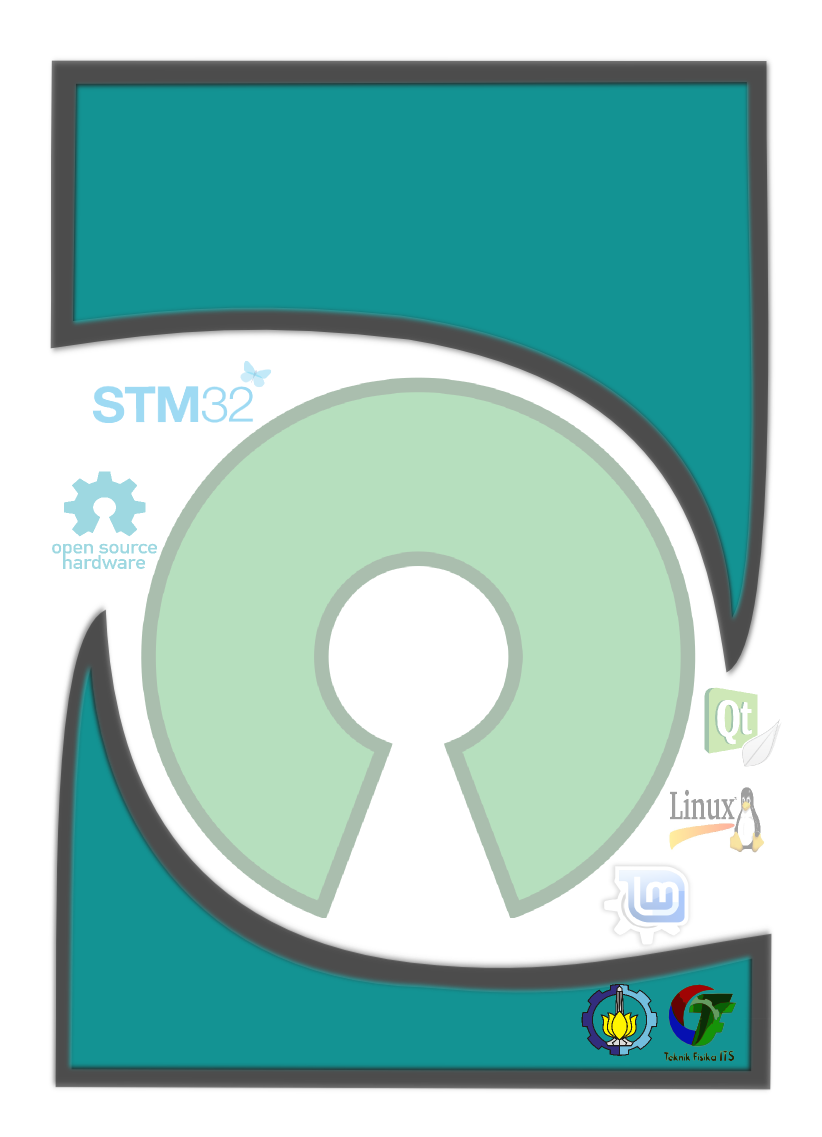
\includegraphics[scale=0.9]{covermodule}}} % Image background
  \end{center}
  \centering
  \vspace*{9cm}
  \par\normalfont\fontsize{35}{35}\sffamily\selectfont
  Pelatihan OpenSources dan STM32\par % Book title
  \vspace*{1cm}
  {\Huge Modul Teknis}\par % Author name
  \vspace*{1cm}
  {\large TF OpenSources}\par
  {\large 2014}\par
\endgroup
% 
\newpage
~\vfill
\thispagestyle{empty}
\noindent Copyright \copyright\ 2014 TF OpenSources\\ % Copyright notice
\noindent \textsc{Published by TF OpenSources}\\ % Publisher
\noindent \textsc{book-website.com}\\ % URL
\noindent Licensed under the Creative Commons Attribution-NonCommercial 3.0 Unported License (the ``License''). You may not use this file except in compliance with the License. You may obtain a copy of the License at \url{http://creativecommons.org/licenses/by-nc/3.0}. Unless required by applicable law or agreed to in writing, software distributed under the License is distributed on an \textsc{``as is'' basis, without warranties or conditions of any kind}, either express or implied. See the License for the specific language governing permissions and limitations under the License.\\ % License information
\noindent \textit{First printing, March 2013} % Printing/edition date

\newpage
\chapterimage{header44.png} % Table of contents heading image
\pagestyle{empty} % No headers
\tableofcontents % Print the table of contents itself
\cleardoublepage % Forces the first chapter to start on an odd page so it's on the right
\pagestyle{fancy} % Print headers again

\newpage
\chapterimage{header46.png} % Chapter heading image
\chapter{OpenSource}
\section{FOSS}
 \hspace{10pt} Foss adalah Free/ Open Source Software dapat diartikan sebagai perangkat lunak atau program komputer yang menyertakan kode program (source code, sehingga disebut sebagai opened source) dan tersedia bebas untuk digunakan, digandakan, dipelajari, dimodifikasi, didistribusi ulang, dan disebarluaskan. 
 Istilah FOSS merupakan gabungan dari Free Software dan Open Source. 
 FOSS yang paling banyak digunakan di berbagai negara di dunia saat ini adalah GNU/ Linux (atau Linux- Kernel)
\section{Open Source}
 \hspace{10pt} Open source adalah sistem pengembangan yang tidak dikoordinasi oleh suatu individu/ lembaga pusat, tetapi dilakukan oleh para pelaku yang bekerja sama dengan memanfaatkan kode sumber (source-code) yang tersebar dan tersedia bebas (biasanya menggunakan fasilitas komunikasi internet). 
 Open source menjamin hak untuk mengakses, memodifikasi kode sumber, menggunakan kembali serta menyebarluaskan perangkat lunak open source  tanpa harus membayar. 
 Linux adalah salah satu open source software.
\section{Lisensi}
%\begin{justified}
 \hspace{10pt} Lisensi secara umum adalah izin untuk menggunakan, mengubah, menggandakan, atau menyebarkan suatu produk tertentu.
 Dalam dunia opensource, pengaturan, pengawasan, dan pengesahan lisensi opensource dilakukan oleh organisasi Open Sources Initiative (OSI).
 Situs resmi OSI dapat diakses di:\\
 \vspace{5pt}
 \url{http://opensource.org/}\\
 \vspace{5pt}
 \hspace{10pt} Berikut adalah daftar lisensi yang telah disahkan dan disarankan oleh OSI:\\
 \itab{- Apache 2.0..}\\
 \itab{- GNU General Public License (GPL) 2.}\\
 \itab{- GNU General Public License (GPL) 3.}\\
 \itab{- GNU Lesser General Public License (LGPL) 2.1.}\\
 \itab{- GNU Lesser General Public License (LGPL) 3.0.}\\
 \itab{- MIT License (MIT)}\\
 \itab{- Mozilla Public License (MPL) 2.0.}\\
 \hspace{10pt} Lebih jauh tentang daftar lisensi yang disahkan OSI dapat dilihat di:\\
 \vspace{5pt}
 \url{http://opensource.org/licenses}\\
 \hspace{10pt} Secara umum lisensi opensources memiliki beberapa poin penting yaitu:\\
 \itab{- Izin untuk menggunakan, mengubah, menggandakan, atau menyebarkan.}\\
 \itab{- Produk tidak memiliki royalti.}\\
 \itab{- Kode sumber atau desain dapat di akses secara publik.}\\
 \itab{- Produk tidak memiliki royalti.}\\
 \itab{- Proyek turunan memiliki lisensi yang sama.}\\
 \itab{- Tidak boleh membuang nama author asli.}\\
 \itab{- Tidak ada diskriminasi.}\\

 
\section{Komersial}
%\begin{justified}
\hspace{10pt} Perlu dicatat bahwa produk yang bersifat komersial berbeda dengan \textit{proprietary}.
Produk yang bersifat \textit{proprietary} memiliki banyak restriksi terutama dari sisi kode sumber dan desain.
Sedangkan opensource bersifat sebaliknya.
Akan tetapi sekalipun tidak ada restriksi di sisi kode sumber dan desain, pengembang tetap dapat menjual produknya.
Penjelasan lebih jauh dapat di lihat di alamt ini:\\
\url{http://opensource.org/faq#commercial}\\
\hspace{10pt} Sebagai contoh adalah produk Arduino, embedded board yang kini sangat populer.
Arduino dirilis dalam lisensi GPL sehingga mahasiswa dapat mengakses desain dan kode sumber baik untuk hardware dan softwarenya.
Namun hardware Arduino tetap dijual dengan harga lumayan mahal dan masih laku.\\
\hspace{10pt} Contoh lain adalah perusahaan Canonical yang menjadi pengembang Ubuntu.
Ubuntu merupakan operating system yang bersifat opensources namun Canonical tetap dapat menghasilkan pendapatan yang besar.
Pendapatan tersebut berasal dari jasa dukungan teknis (namun masih lebih mahal dukungan teknis Microsoft Corp.) maupun jasa penyewaan hardware dan server berbasis Ubuntu.


\section{Bajakan}
\begin{flushleft}
\hspace{10pt} Dampak negatif menggunakan software bajakan:\\
\itab{- Software bajakan tidak 100\% serupa dengan software yang asli.}\\
\itab{- Memiliki efek samping yang buruk pada kinerja dan fungsi PC.}\\
\itab{- Penggunaan software bajakan bisa menghemat uang untuk jangka pendek, namun dari segi}\\
\itab{\hspace{6pt}keamanan PC tidak terjamin.}\\
\itab{- Software bajakan tempat bersarangnya malware, yaitu aplikasi computer yang khusus dibuat}\\
\itab{\hspace{6pt}dengan tujuan mencari kelemahan software.}\\
\itab{- Membajak software tergolong mencuri atau menggunakan tanpa hak}\\
\itab{- Dalam Islam hukumnya haram serta berdosa besar jika dilakukan terus tanpa bertaubat.}\\
\end{flushleft}

\newpage
\chapterimage{headerbiru3.jpg} % Chapter heading image
\chapter{LinuxMintKDE}
\section{Linux}
%\begin{justified}
\hspace{10pt}Linux adalah salah satu sistem operasi varian unix yang merupakan salah satu saingan terbesar Microsoft Windows. 
Linux merupakan sistem operasi yang open source dibawah lisensi GNU GPL \textit{(Gnu is Not Unix) General Public License (GPL)} sehingga gratis dan kita bisa memperoleh \textit{sourcecode} nya. 
Linux kuat karena didukung oleh komunitasnya yang sangat banyak. 
Namun karena Linux bersifat open source tadi maka linux pun mudah dikembangkan oleh siapa saja. 
Distribusi linux dapat berupa perangkat lunak bebas dan dapat pula berupa perangkat lunak komersial.
Berikut ini adalah distribusi linux yang paling populer :\\
\itab{-\hspace{8pt}\textbf{Arch Linux}, merupakan distribusi jenis rolling release yang ditargetkan pada pengguna Linux }\\
\itab{ \hspace{8pt}yang sudah berpengalaman, Arch Linux dikelola oleh sebuah komunitas.}\\
\itab{-\hspace{8pt}\textbf{Debian}, distribusi ini dikelola oleh sukarelawan di komunitas. Berikut ini merupakan contoh}\\
\itab{ \hspace{8pt}distribusi populer yang diturunkan dari Debian.}\\
\itab{\hspace{10pt}- \hspace{8pt}\textbf{Canamia}}\\
\itab{\hspace{10pt}- \hspace{8pt}\textbf{Knoppix}}\\
\itab{\hspace{10pt}- \hspace{8pt}\textbf{Ubuntu}, merupakan distribusi yang paling popular yang berasal dari debian, dikembangkan}\\
\itab{\hspace{12pt}\hspace{8pt} oleh perusahaan Canonical Ltd. Perkembangan Ubuntu diantaranya adalah Linux Mint,}\\
\itab{\hspace{12pt}\hspace{8pt} Lubuntu, Xubuntu, Kubuntu, dll. }\\
\itab{-\hspace{8pt}\textbf{Fedora}, distribusi komunitas yang disponsori oleh perusahaan Amerika, RedHat yang bersifat}\\
\itab{\hspace{8pt} komersil.}\\
\textbf{Mengapa Harus Menggunakan LINUX?}\\
\itab{-\hspace{8pt}Karena Linux gratis sehingga tidak memerlukan lisensi.}\\
\itab{-\hspace{8pt}Karena Linux juga seperti Windows, memiliki GUI yang juga semakin bagus. Tidak hanya itu}\\
\itab{\hspace{8pt}\hspace{2pt}sekarang Linux juga sudah sangat kompatibel dengan hardware- hardware baru seperti flashdisk}\\
\itab{\hspace{8pt}\hspace{2pt}dan bluetooth.}\\
\itab{-\hspace{8pt}Semua yang bisa dijalankan di Windows, rata- rata ada juga di Linux dan semuanya GRATISS!!}\\
\itab{-\hspace{8pt}Linux bisa diinstall bersamaan dengan Windows pada harddisk yang sama maupun berbeda.}\\
\itab{\hspace{8pt}\hspace{2pt}Bahkan ada yang bisa diinstall bersamaan di partisi Window.}\\
\itab{-\hspace{8pt}Linux sangat stabil dan sangat cocok jika dijadikan server.}\\
\itab{-\hspace{8pt}\textbf{ANTI VIRUS!!}}\\
\begin{center}
 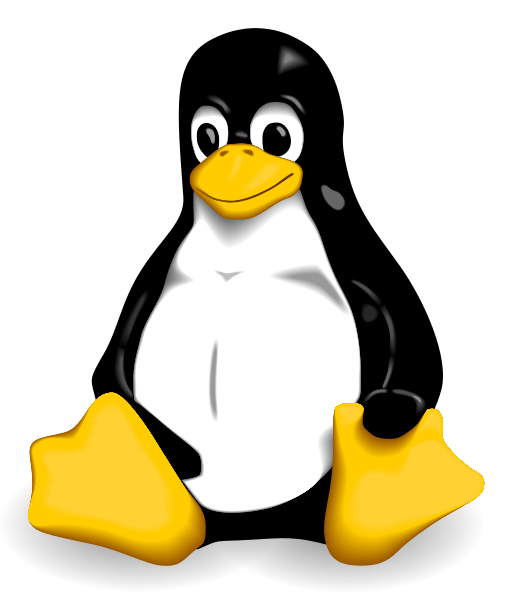
\includegraphics[width=4cm,height=4cm]{linux.png}\\
  \textbf{Icon Linux}
\end{center}
\section{KDE}
\hspace{10pt} KDE (K Dekstop Environmental) adalah lingkungan dekstop (dekstop environment), karena banyak yang mengatakan linux hanya sistem operasi yang hanya berkutat di mode teks saja, setiap akan menjalankan aplikasi kita harus mengetikan perintah di dalam shell/ terminal/ konsole maka linux menyediakan lingkungan grafis yang disebut dengan Dekstop Environment (DE). 
KDE adalah salah satu dari jenis Dekstop eviroment. Berikut ini adalah beberapa jenis Dekstop Environment :\\
\itab{- Unity, dipakai di Ubuntu}\\
\itab{- GNOME, dipakai di Ubuntu GNOME}\\
\itab{- KDE, dipakai di Ubuntu, Linux Mint, dll}\\
\itab{- LxDE, dipakai di Lubuntu}\\
\itab{- Mate, dipakai di Ubuntu Mate}\\
\itab{- XFCE, dipakai di Xubuntu}\\
\section{UNIX}
\hspace{10pt} Antara linux dan unix keduanya merupakan OS Open Source yang dapat memungkinkan terjadinya perubahan kode.
Segi keamanan Linux dianggap lebih efisien dalam hal mendeteksi ancaman virus. 
Hal itu karena linux merupakan sistem operasi masyarakat, jadi setiap kali user menemukan virus ia melapor kepada masyarakat dan pengembang sistem operasi membantunya.
Sedangkan UNIX merupakan sistem operasi user harus menunggu untuk patch anti-virus dari produsen.
Sehingga dapat dikatakan bahwa dalam segi keamanan Linux dapat dinilai lebih unggul dari UNIX.\\
\hspace{10pt} Unix adalah kernel yang dikembangkan bersamaan dengan bahasa C dan merupakan kernel komputer modern yang paling tua.
Dari kernel Unix inilah turun sistem operasi MacOS, Linux, Minix, BSD, DOS, MS-DOS, dan Windows.
Saat ini Unix sendiri masih digunakan untuk komputer-komputer khusus di perusahan besar seperti IBM dan HP.
Lisensi Unix sendiri yang \textit {teproprietary} (hak milik) dan mahal harganya, membuat Unix tidak luas penggunaanya.
\section{Debian/Ubuntu}
\hspace{10pt} Debian adalah sistem operasi komputer yang tersusun dari paket- paket perangkat lunak yang dirilis sebagai perangkat lunak bebas dan terbuka denga lisensi mayoritas GNU General Public License. 
Ubuntu merupakan salah satu distribusi Linux yang berbasiskan Debian dan didistribusikan sebagai perangkat lunak bebas, tidak ada biaya lisensi, pengguna memiliki kebebesan untuk mengubah sesuai dengan kebutuhan komputasi pengguna. 
Lisensi yang pada umumnya adalah GNU General Public License (GNU GPL) dan GNU Lesser General Public License (GNU LGPL), dengan tegas menyatakan bahwa pengguna dengan bebas dapat menjalankan, menggandakan, mempelajarai, memodifikasi, dan mendistribusikan tanpa pembatasan apapun. Namun tetap ada software proprietary (hak milik) yang dapat berjalan di Ubuntu. 
Dalam hal keamanan, perangkat sudo dapat meningkatkan privilage secara sementara untuk melakukan tugas administratif, sehingga akun root dapat terus terkunci, dan mencegah orang tidak terauthorisasi melakukan perubahan sistem atau membuka kelemahan keamanan. 
\section{LinuxMint}
\hspace{10pt} OpenSource for Embedded Development Training ini menggunakan Sistem Operasi Linux Mint, dimana linux mint adalah salah satu sistem operasi Linux yang masih keturunan Ubuntu. 
Kelebihan linux Mint dibandingkan dengan distro linux lain adalah kemudahan penggunaan, bahkan oleh seorang pengguna komputer awan pun akan dengan mudah beradaptasi dengan Linux Mint. 
Linux Mint memungkinkan di-install di dalam Windows sebagai sebuah perangkat lunak biasa. 
Berbeda dengan Ubuntu, Linux Mint hadir dengan dukungan playback file multimedia dan flash player, hal ini tidak terdapat di Ubuntu Linux. 
Linux Mint rilis sebanyak dua kali dalam setahun. Setiap rilis Linux Mint diberi nama versi dan code name yang memakai nama- nama wanita dan selalu berakhiran ‘a’ (contoh Linux Mint 17.1 Rebecca, 17 .1 adalah nomor versi dan Rebecca adalah code name yang berakhiran ‘a’)\\
Pada “Open Source for Embedded Development Training” menggunakan Linux Mint 17 Qiana KDE.\\
\begin{center}

\includegraphics[width=4cm,height=4cm]{MINT1.jpg}\\
  \textbf{Linux Mint}
\end{center}
\section{Dolphin}
\hspace{10pt} Pengguna yang terbiasa menggunakan Windows pasti mengetahui Windows Explorer. 
Aplikasi ini berfungsi untuk mengatur berbagai macam file, mulai dari dokumen teks, foto, audio, video, dan banyak lagi. 
Sama dengan Windows, Kubuntu juga memiliki aplikasi pengelola file yang disebut dengan Dolphin.\\ 
\begin{center}
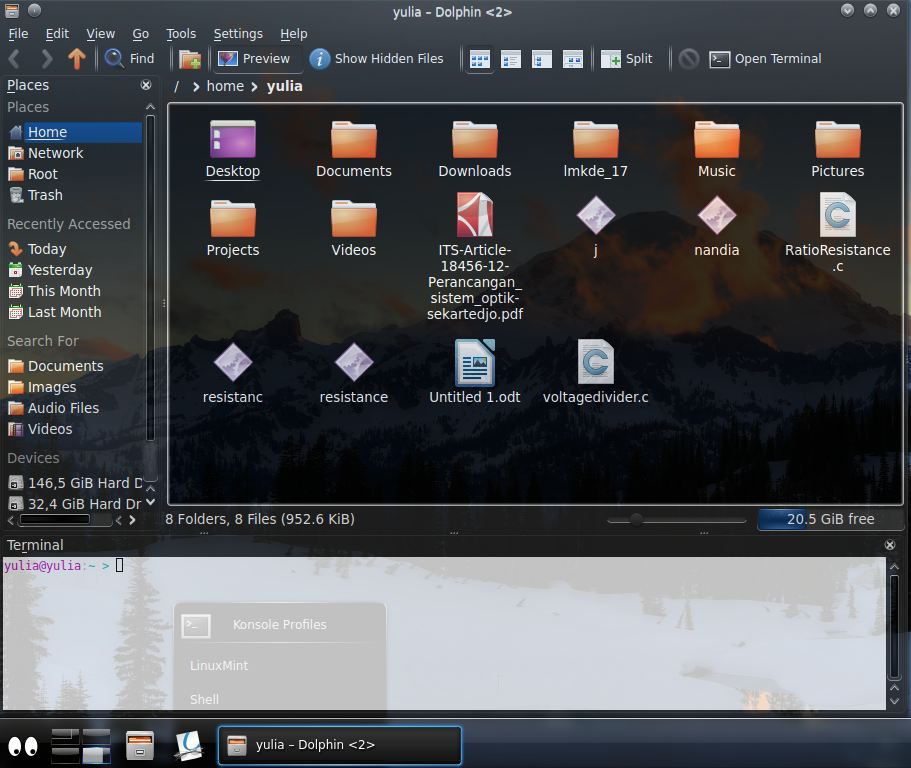
\includegraphics[width=14cm,height=10cm]{dolphin.png}\\
\textbf{Tampilan Dolphin seperti Windows Eksplore}
\end{center}
\section{Konsole}
\hspace{10pt} Konsole adalah sebuah shortcut yang dapat digunakan untuk menjalankan perintah- perintah tertentu pada OS Linux, kalau dalam Windows biasanya disebut DosPrompt. 
Pada konsole(terminal) dapat menjalankan perintah yang kita inginkan secara otomasti. Contohnya membuat folder (directory) dengan meginputkan code nya. 
Gambar dibawah ini adalah contoh membuat folder (directory) dengan nama folder 'kuliah', dengan meninputkan kode 'mkdir kuliah' maka akan terbentuk folder kuliah.
mdir kuliah artinya, make directory kuliah. Cara menghapus folder dengan mengetik 'rmdir kuliah' artinya, remove directory, maka folder kuliah akan terhapus.
\begin{center}
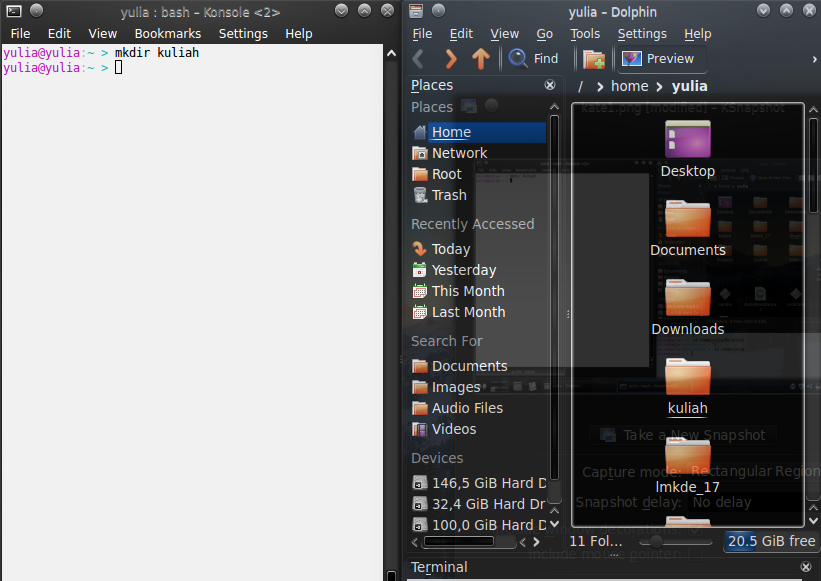
\includegraphics[width=14cm,height=9cm]{konsole.png}\\
\textbf{Membuat Directory Kuliah}\\
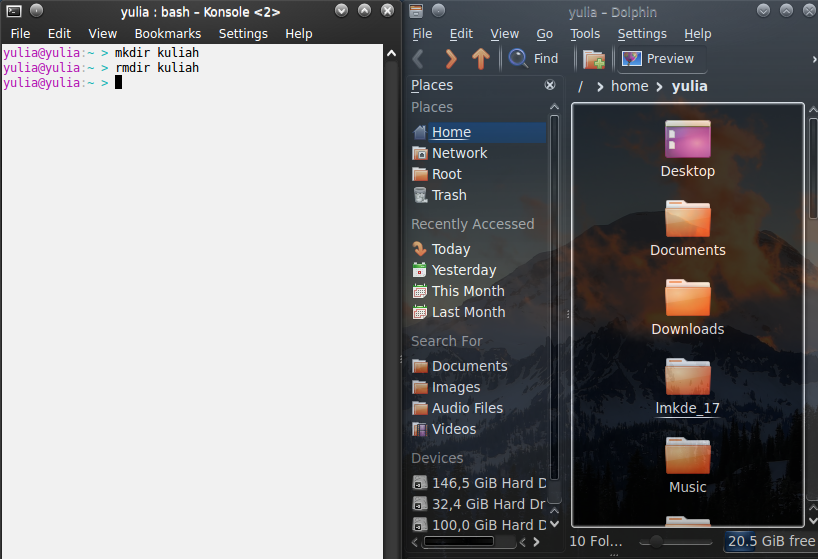
\includegraphics[width=14cm,height=9cm]{konsole1.png}\\
 \textbf{Menghapus Directory Kuliah}\\
\end{center}
\section{Mozilla Firefox}
\hspace{10pt}Mozilla Firefox adalah sebuh aplikasi browsing yang sangat popular dibuat oleh mozilla coorporation, firefox adalah salah satu web browser open source. 
\section{Kate}
\hspace{10pt} Kate adalah editor teks dimana editor teks berfungsi untuk membuat file teks yang dapat berupa teks biasa maupun sebuah skrip. 
Sistem operasi Linux dibekali dengan 2 mode editor, yang pertama adalah editor berbasis teks (vi, emacs, dll) dan yang kedua adalah editor berbasis grafis (mousepad, gedit, kate, dll). 
Gambar dibawah ini adalah tampilan kate berupa skrip.\\
\begin{center}
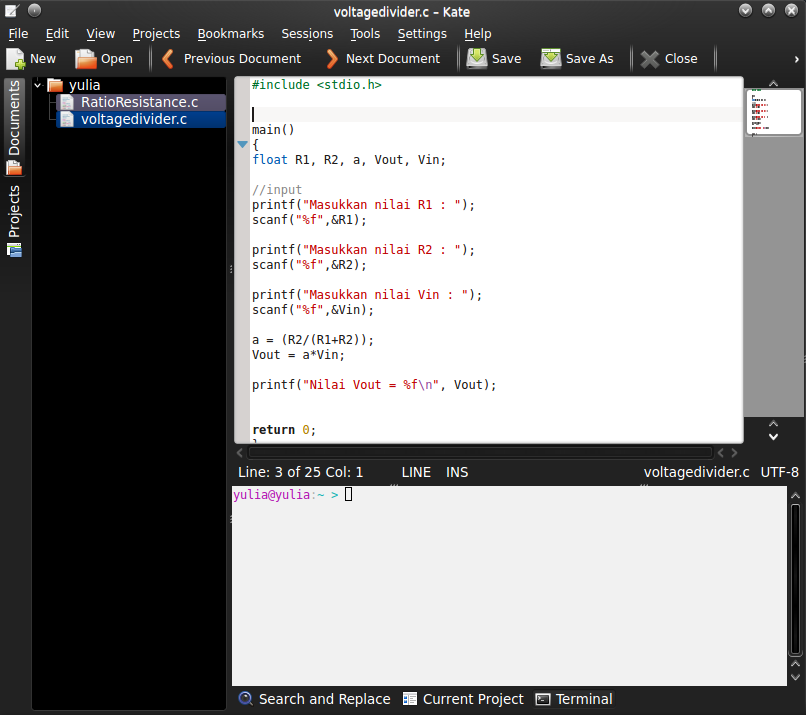
\includegraphics[width=14cm,height=10cm]{kate.png}\\
\textbf{Kate Untuk Membuat File Berupa Skrip}\\
\end{center}
\section{Kile}
\hspace{10pt} Kile adalah editor LaTeX yang berjalan pada desktop KDE. 
Latex adalah sistem penyiapan dokumen untuk peranti lunak TeX, TeX merupakan program komputer yang digunakan
untuk typesetting suatu dokumen atau membuat formula matematika.\\
Untuk menjalankan Kile memerlukan  beberapa komponen yang harus terinstal dalam sistem, yaitu:\\ 
\itab{-\hspace{8pt}K Desktop Environment (KDE)}\\
\hspace{20pt}KDE adalah desktop environment yang cukup populer di dunia open source (Minimal KDE 3).\\
\itab{-\hspace{8pt}Qt, Qt adalah tool C++ yang berguna untuk melakukan kompilasi kile.}\\
\itab{-\hspace{8pt}LaTeX: Program typesetting dokumen yang berkualitas tinggi. Kebanyakan LaTeX yang}\\
\itab{\hspace{8pt}digunakan pada lingkungan Unix atau Linux adalah distribusi LaTeX.}\\
Pembuatan modul “Open Source for Embedded Development Training” menggunakan Kile. \\
\begin{center}
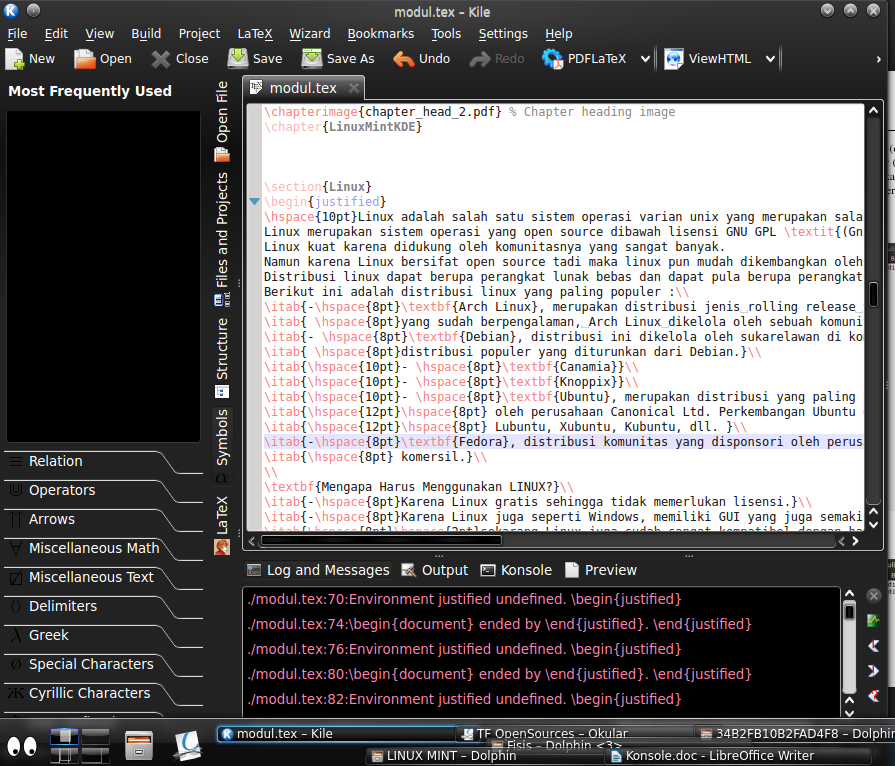
\includegraphics[width=14cm,height=10cm]{kile.png}\\
\textbf{Modul “Open Source for Embedded Development Training” Menggunakan Kile}
\end{center}
\section{LibreOffice}
\hspace{10pt} LibreOffice adalah sebuah paket aplikasi perkantoran yang kompatibel dengan aplikasi perkantoran seperti Microsoft Office. 
LibreOffice sebagai perangkat lunak yang bebas dan gratis. 
LibreOffice merupakan proyek pengembangan dari OpenOffice. 
OpenOffice sama-sama aplikasi perkantoran yang bersifat gratis, tetapi setelah itu OpenOffice dibeli oleh oracle dan produk pengembangannya adalah LibreOffice.  
Semua fitur yang ada di OpenOffice ada pula di LibreOffice. 
Open Office dan Libre Office dapat berjalan di sistem operasi Microsoft Windows dan Linux. 
Sebagaimana Microsoft Office, Open Office dan Libre Office memiliki aplikasi pengolah kata, spreadsheet, basis data, dan presentasi. 
Tampilan wajah aplikasi-aplikasi Open Office dan Libre Office juga tidak jauh berbeda dengan Microsoft Office. 
\section{GIMP}
\hspace{10pt}
GIMP (GNU Image Manipulation Program) adalah perangkat lunak yang berbasis bitmap,seperti Photoshop. 
Program ini merupakan perangkat lunak yang didistribusikan secara gratis dapat digunakan untuk beberapa keperluan, misalnya mengolah foto, mengomposisi gambar (citra), dan membuat gambar. 
GIMP merupakan salah satu program grafis yang mempunyai beragam kemampuan. 
Program ini dapat digunakan sebagai suatu program gambar sederhana, program pengolah foto yang sangat baik, suatu sistem yang dapat diproses secara online, membuat gambar berskala besar, konversi format gambar, dan lain-lain.
% %\end{justified}
\section{Inkscape}
\hspace{10pt} Inkscape adalah perangkat lunak berbasis vektor (\textit{Software Vector Graphics}), seperti CorelDraw, yang sifatnya OpenSource dibawah lisensi linux GNU GPL (GNU General Public License) sehingga gratis dan tidak berbayar seperti CorelDraw. 
Kelebihan Inkscape dibandingkan dengan CorelDraw adalah sebagai berikut:\\
\itab{- Instalasi font lebih mudah}\\
\itab{- Komponen warna lebih kaya}\\
\itab{- Gradasi lebih cermat}\\
\itab{- Dapat mengatur \textit{Oppacity} dan \textit{blur}\, ini yang menyebabkan warna- warna diinkscape lebih bervariasi}\\
\itab{- Vektor buatan inkscape (.svg) dapat dibuka di CorelDraw (.cdr)}\\
\itab{- GRATIS! Bisa dikembangkan maupun disebarluaskan}\\
Pembuatan poster “Open Source for Embedded Development Training “ menggunakan Inkscape.\\
\begin{center}

\includegraphics[width=5cm,height=5cm]{1.jpg}\\
  \textbf{Inkscape}
\end{center}
\section{EAGLE}
\hspace{10pt}Eagle \textit({Easily Applicable Graphical Layout Editor}) merupakan sebuah aplikasi gratis untuk mendesain skema elektronika maupun PCB (Printed Circuit Board). 
Aplikasi Eagle ini kita bisa merancang, memodifikasi, dan mencetaknya untuk kemudian disablon ke dalam bentuk PCB. Aplikasi ini tersedia untuk sistem operasi GNU/Linux, Macintosh, maupun Ms. Windows. 
Pada Open Source for Embedded Development Training software eagle digunakan untuk mendesain jalur circuit pada board yang digunakan untuk menyambungkan mikrokontroler STM32, downloader, dll.
\newpage
\chapterimage{headerbiru22.png} % Chapter heading image
\chapter{Tools Chain}
\section{Qt}
\hspace{10pt}Software Qt adalah User Interface framework dan editor yang ditulis dengan bahasa C++ namun penggunaan bahasa lain seperti C, Java, Python juga didukung melalui Binding dapat dilakukan di Qt. 
Qt dipakai untuk membuat interface atau membuat KDE beserta aplikasi- aplikasinya. Qt seperti Visual Basic pada windows yang digunakan untuk membuat interface dan seperti kate pada Linux yang digunakan sebagai editor. 
Aplikasi ternama yang dikembangkan dengan menggunakan Qt framework diantaranya Google Earth Map application, Skype, VLC media player, KDE desktop Environment, dll.
Qt pada pelatihan ini digunakan sebagai editor library yang ada pada ChibiOS.
\section{ChibiOS}
\hspace{10pt}Adalah salah satu jenis Real Time Operating System (RTOS).  
RTOS adalah sistem operasi yang digunakan sebagai kontrol dari suatu devais berdasarkan waktu. 
RTOS relatif lebih cepat daripada operating system biasa yang kita gunakan (Windows, Linux, Mac). RTOS digunakan untuk sistem operasi untuk mikrokontroler. 
Jadi, yang ditanamkan di dalam mikrokontroler STM32 nanti adalah operating system real time (RTOS) jenis ChibiOS, ChibiOS ini terdiri dari library- library yang nantinya library ini akan diedit sesuai kebutuhan kita di editor, yaitu Qt (sudah dijelaskan diatas).
%\section{GCC ARM EABI}
\section{GCC (GNU Compiler Collection)}
\hspace{10pt} Kompiler adalah sebuah program komputer yang berguna untuk menjalankan program komputer yang ditulis dalam pemrograman bahasa C++, C, Visual Basic, dll.  
GCC (GNU Compiler Collection) adalah sebuah kompiler yang khusus bekerja untuk bahasa pemrograman C yang dikembangkan oleh komunitas GNU project. 
GCC digunakan untuk meng-compile program pada PC/laptop. 
Pada “Open Source for Embedded Development Training” ini library yang ada pada ChibiOS akan di edit sesuai kebutuhan pada editor Qt, lalu akan di compile dengan GCC. 
\section{GCC ARM EABI}
\hspace{10pt}GCC ARM EABI adalah compiler untuk mikrokontroler ARM.
 Jadi program yang sudah kita buat perlu dicompile dengan GCC ARM EABI agar bisa dijalankan dan setelah itu ditanam di mikrokontroler STM 32.
\section{Program Downloader}
\hspace{10pt} Program downloader digunakan untuk menanankam program yang sudah kita buat di PC ke mikrokontoler, atau dapat disebut sebagai jembatan penyambung komputer dan mikrokontolernya. 
Jenis program downloader ada bermacam-macam, diantaranya :\\
1. USBasp adalah salah satu downloader yang support untuk atmel mikrokontroller yang penggunanya memakai SPI.
SPI (Serial Pheripheral Interface) merupakan salah satu mode komunikasi serial synchrounous kecepatan tinggi
yang dimiliki oleh ATmega. Komunikasi SPI membutuhkan
3 jalur yaitu MOSI, MISO, dan SCK. Melalui komunikasi data ini
data dapat saling dikirimkan baik antar mikrokontroler maupun antara mikrokontroler dengan peripheral lain di luar mikrokontroller.\\
2. Uart flash adalah UART (Universal Asynchrounous Receiver- Transmitter) sebuah mode komunikasi
serial secara asynchronous, dimana data dikirim secara satu persatu melalui kabel
ganda (twisted pair Tx dan Rx). Pada ``Open Source for Embedded Development Training''
menggunakan jenis komunikas UART, dengan bantuan FTDI.
\newpage
\chapterimage{headerbiru22.png} % Chapter heading image
\chapter{Mikrokontroler}
\section{Gambaran Umum}
\hspace{10pt}Seperti yang kita ketahui bahwa Robot line tracer terdiri dari dua buah jenis yaitu analog dan digital (yang dilombakan di acara EPW Teknik Fisika). 
Jika robot line tracer analog tidak  perlu mikrokontroler, ataupun software yang lainnya, sedangkan robot line tracer digital dituntut untuk dapat menggunakan software dalam pengoprasian robot dengan mikrokontroler.
Software yang digunakan pada robot line tracer digital, yaitu : \\
\itab{- Software bahasa pemrograman, bahasa pemrograman yang digunakan mulai dari bahasa yang}\\
\itab{\hspace{2pt} sulit seperti assembly, pascal, atau yang biasa digunakan yaitu bahasa basic dan C.}\\ 
\\
\itab{- Software downloader mikro, adalah perangkat lunak yang berfungsi memasukan program}\\
\itab{\hspace{2pt}ke dalam mikrokontroler (STM32). Software downloader mikro yang kita gunakan pada}\\
\itab{\hspace{2pt}pelatihan ini berbasis komunikasi Uart flash dengan bantuan chip FTDI. FTDI berasal dari}\\
\itab{\hspace{2pt}nama perusahaan pembuat chip.}\\
\\
\hspace{10pt}Cara kerja dari sistem robot line follower secara umum ialah dimulai dari pembacaan lintasan atau garis oleh sensor photodiode berserta LED superbright yang mana intensitas pantulan sinar LEDsuperbright 
akan berbeda jika terkena bidang pantul yang gelap dengan bidang pantul yang lebih terang, dari perbedaan inilah dimanfaatkan sebagai pendeteksi lintasan atau garis dan selanjutnya diteruskan pada rangkaian untai pengkondisi sinyal (komparator). 
Hasil keluaran komparator kemudian diteruskan dan diproses oleh rangkaian pengendali utama yakni IC mikrokontroler (contoh STM32). 
Pada bagian kendali utama inilah semua logika pembacaan sensor yang telah dikondisikan oleh komparator diproses.\\
\\
\hspace{10pt}Bagian mikrokontroler ini terdiri dari dua masukan dan dua keluaran. 
Pada bagian masukan berupa sensor dengan untai komparator dan keypad kendali yang berfungsi untuk mengatur 
algoritma kendali yang akan digunakan pada robot line follower. 
Pada bagian keluaran berupadisplay (penampil) dengan menggunakan LCD dan PWM 
mikrokontroler STM 32 yang diteruskan ke driver motor, untuk mengendalikan motor kiri dan kanan dari robot line tracer.
\section{ARM Cortex- M3 Processor}
\hspace{10pt}Adalah sebuah desain prosesor berarsitektur RISC karya perusahaan ARM Holdings. 
Perusahaan ARM Holdings didirikan pada tahun 1990 dengan nama Advanced RISC Machines, 
sebuah perusahaan patungan anatara Acorn Computers, Apple Computer (sekarang Apple.Inc) dan VLSI Technology. 
ARM fokus pada penelitian dan pengembangan desain arsitektur prosesor. 
Tidak seperti intel dan AMD (arsitektur berbasis CICS, yang biasanya digunakan pada prosesor untuk PC) yang memproduksi dan menjual prosesor, 
ARM menjual lisensi hak kekayaan intelektual atau hak paten desain prosesor kepada perusahaan pemanufaktur semikondukor seperti Qualcomm, Nvidia, Texas Instrument, dll 
bahkan Intel dan AMD pun membeli lisensi desain ARM. 
Aristektur ARM dijadikan landasan bagi sebagian Central Processing Unit (CPU) dikebanyakan perangkat mobile sekarang ini. Hampir semua tablet dan ponsel pintar unggul,
baik berbasis Android, iOS, BlackBerry, hingga Windows Phone, memakai prosesor arsitektur ARM. ARM mempunyai desain arsitektur Cortex Seri M, R, A, hingga seri A50. 
ARM Cortex-M3 Processor 32 bit ini adalah prosesor 32 bit yang secara khusus dikembangkan untuk pengembangan mikrokontroler, otomotif sistem, 
sistem kontrol industri, dan jaringan nirkabel dan sensor. Prosesor ini memiliki kinerja komputasi yang luar biasa dan respon sistem yang luar biasa. 
\section{STM 32}
\hspace{10pt}STM 32 adalah mikrokontroler 32 bit berbasis ARM Cortex-M yang dikembangkan untuk embedded system. 
\section{ChibiOS}
\hspace{10pt}Adalah salah satu jenis Real Time Operating System (RTOS). 
RTOS adalah sistem operasi yang digunakan sebagai kontrol dari suatu devais berdasarkan waktu. 
RTOS relatif lebih cepat daripada operating system biasa yang kita gunakan (Windows, Linux, Mac). 
RTOS digunakan untuk sistem operasi untuk mikrokontroler. 
Jadi, yang ditanamkan di dalam mikrokontroler STM32 nanti adalah operating system real time (RTOS) 
jenis ChibiOS, ChibiOS ini terdiri dari library- library yang nantinya library ini akan diedit 
sesuai kebutuhan kita di editor, yaitu Qt (sudah dijelaskan diatas).
\section{Serial Shell ChibiOS }
\hspace{10pt}Serial Shell ChibiOS maksudnya adalah menjalankan library chibiOS pada shell (terminal) yang ada di pc atau laptop yang terhubung langsung dengan mikrokontroler (STM 32). 
Sedangkan  GCC atau G++ yang dibahas seblumnya adalah meng-compile program yang terhubung langsung dengan prosesor komputer, 
sedangkan Serial Shell ChibiOS langsung terhubung pada mikrokontorelnya.
\section{GPIO ChibiOS}
\hspace{10pt}General-purpose input/output (GPIO) adalah pin generik pada sirkuit terpadu (chip) yang perilakunya (termasuk apakah pin itu input atau output) dapat dikontrol (diprogram) oleh pengguna saat berjalan. Ide dibalik GPIO adalah untuk memenuhi sistem integrator dalam memperluas dan membangun sistem lengkap yang membutuhkan pin tambahan dari chip berupa sinyal kontrol ataupun data. 
Adanya konektor (pin) yang tersedia dari chip dapat menghemat kerumitan saat mengatur sirkuit tambahan.
\section{PWM ChibiOS}

\hspace{10pt}PWM ChibiOS adalah generic PWM (Pulse Width Modulation) driver.
HAL (hardware abstraction layer) pada ChibiOS sangat mudah membangkitkan Pulse Width Modulation (PWM).
Indikator sinyal yang dibangkitkan terlihat dari nyala LED yang terang redup pada STM32 Discovery Board.
Pada robot line tracer pulsa PWM berfungsi mengatur kecepatan motor DC, mengatur gelap terang LED dan aplikasi lainnya. 
PWM adalah Timer mode Output Compare yang canggih. 
Mode PWM Timer juga dapat mencacah turun yang berlawanan dengan mode Timer lainnya yang hanya mencacah naik.\\
\chapterimage{headerbiru22.png} % Chapter heading image
\chapter{How to Install}
\section{Partisi Harddisk}
\hspace{10pt}Sebelum menginstal linux perlu dilakukan partisi harddisk. 
Kegunaan dari partisi adalah untuk memberikan space kosong yang akan digunakan sebagai memori ketika kita menginstal linux. 
Aplikasi memori yang kosong dapat kita partisi menjadi beberapa bagian lagi sesuai dengan keinginan kita. 
Hasil dari partisi ini nantinya akan berfungsi seperti memori yang ada pada windows. 
Langkah pertama untuk melakukan partisi pada disk anda adalah sebagai berikut ini:\\
1. Ketik partition pada start button anda\\
\begin{center}
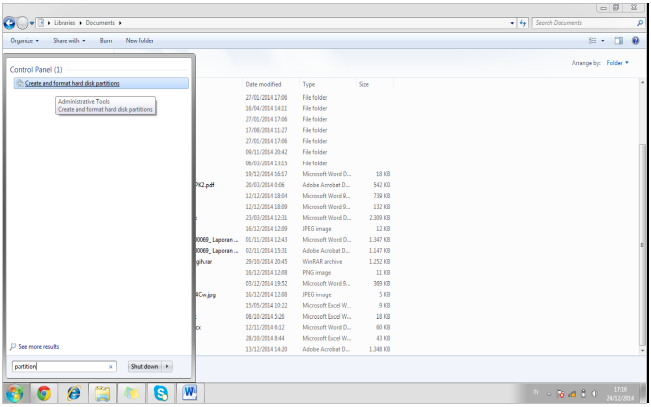
\includegraphics[width=14cm,height=10cm]{partisi1.png}\\
\end{center}
2. Pilih disk yang akan anda partisi, pastikan disk yang anda alokasikan untuk menginstal linux\\
\itab{\hspace{12pt}tidak lebih besar dari kapasitas kosong dari disk yang anda pilih. Jika tidak maka sebagian}\\
\itab{\hspace{12pt}file di disk anda akan terformat.}\\
3. Agar lebih aman, kosongkan disk yang akan anda partisi sehingga data anda tetap aman ketika\\
\itab{\hspace{12pt}terjadi sesuatu hal yang tidak diinginkan.}\\
4. Selanjutnya click kanan pada bagian disk yang akan anda partisi, dan pilih shrink volume\\
\begin{center}
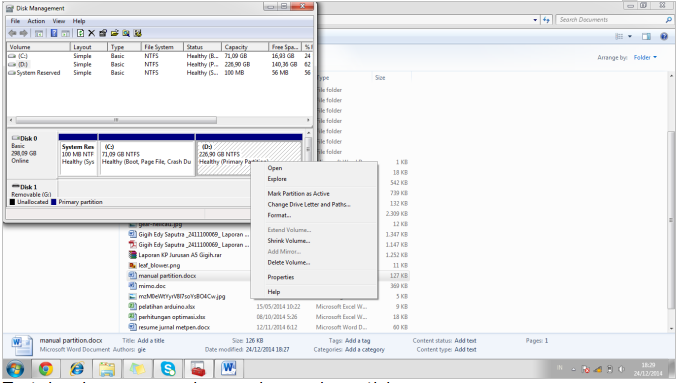
\includegraphics[width=14cm,height=10cm]{partisi2.png}\\
  \end{center}
5. Tentukan besar memori yang akan anda partisi.\\
6. Setelah partisi selesai maka akan ada part dari sisa memori yang telah anda partisi, hapus part\\
\itab{\hspace{12pt}tersebut agardiakumulasikan  dengan memori yang lain}
\section{Instal LInux Mint KDE}
Setelah mempartisi harddisk space kosong akan digunakan sebagai memori ketika kita menginstal linux.
Berikut ini adalah langkah- langkah menginstall linux mint:\\
1. Buka file UUI (Universal USB Installer) pada harddisk atau flasdisk yang tersedia
\begin{center}
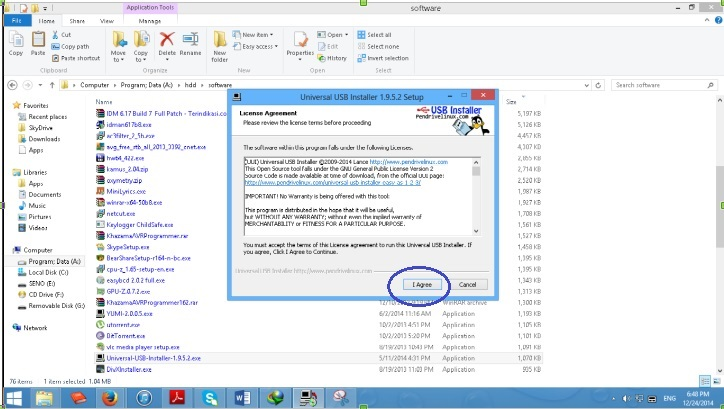
\includegraphics[width=14cm,height=10cm]{uui.jpg}\\
  \textbf{Buka Universal USB Installer}
  \end{center}
2. Setelah itu akan muncul tampilan seperti dibawah ini. Step 1 Pilih distro linux yang akan diinstall, pilih Linux Mint. 
Step 2 cari letak Linux Mint-17-kde-DVD-32 bit.iso. Step 3 pilih USB Flash tempat installer linux, pada contoh gambar dibawah ini terletak pada USB flash 3GB, 
lalu klik create\\
\begin{center}
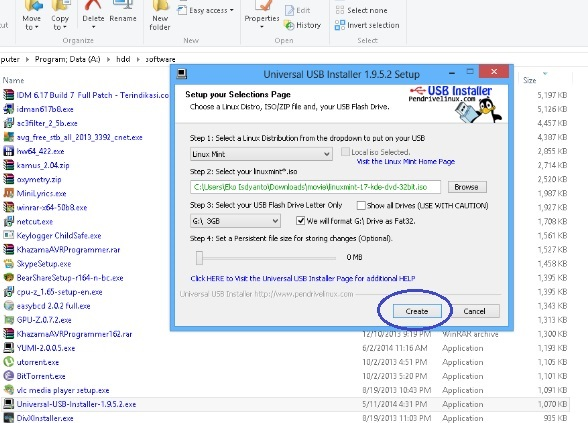
\includegraphics[width=14cm,height=10cm]{ekstrak2.jpg}\\
  \end{center}
  \vspace{2cm}
3. Setelah itu muncul tampilan gambar dibawah ini dan windows akan ter-restart\\
\begin{center}
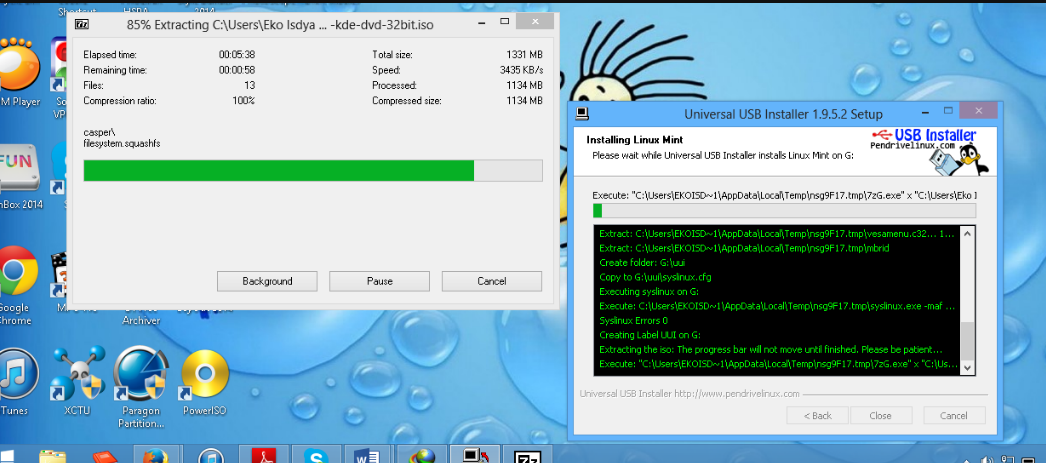
\includegraphics[width=14cm,height=9cm]{ekstrak.png}\\
\end{center}
\vspace{2cm}
4. Klik Install, Lalu ikuti tahapan seperti gambar dibawah ini dengan menekan continue\\
\begin{center}
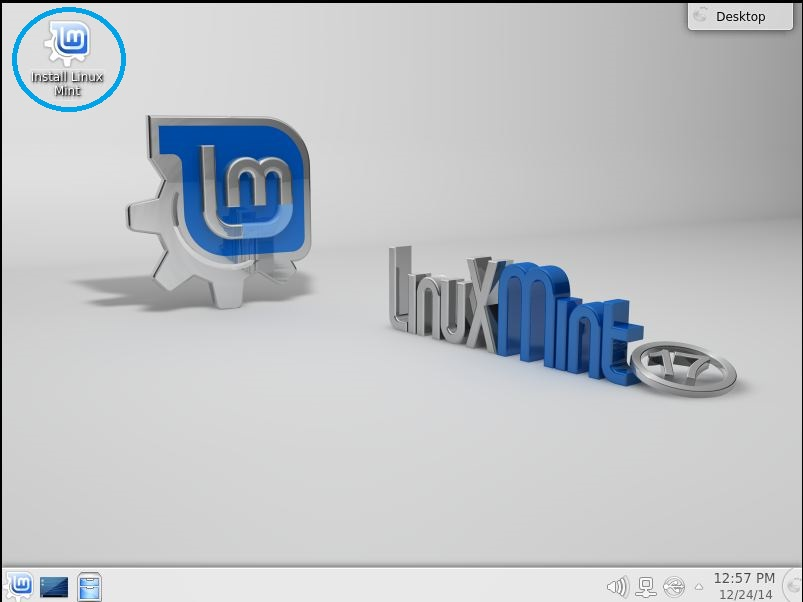
\includegraphics[width=14cm,height=9cm]{Capture1.JPG}\\
\end{center}
\begin{center}
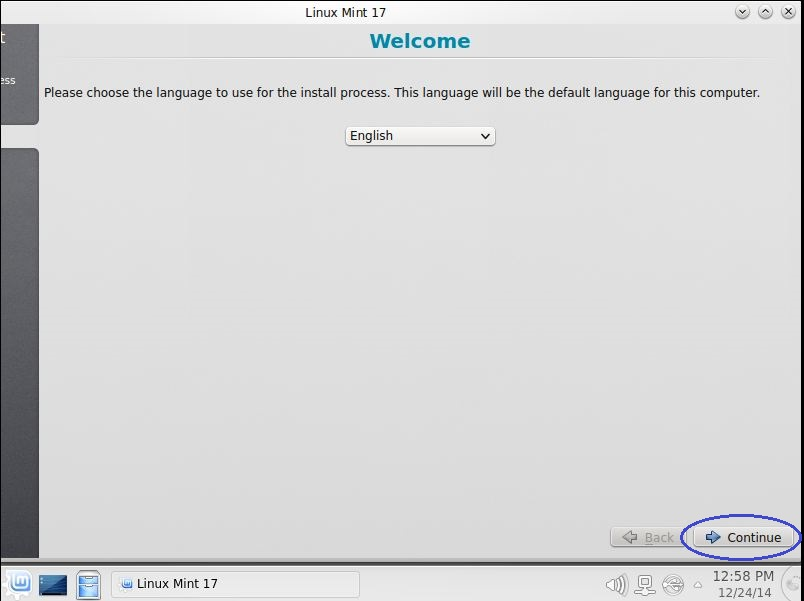
\includegraphics[width=14cm,height=9cm]{Capture2.JPG}\\
\vspace{2cm}
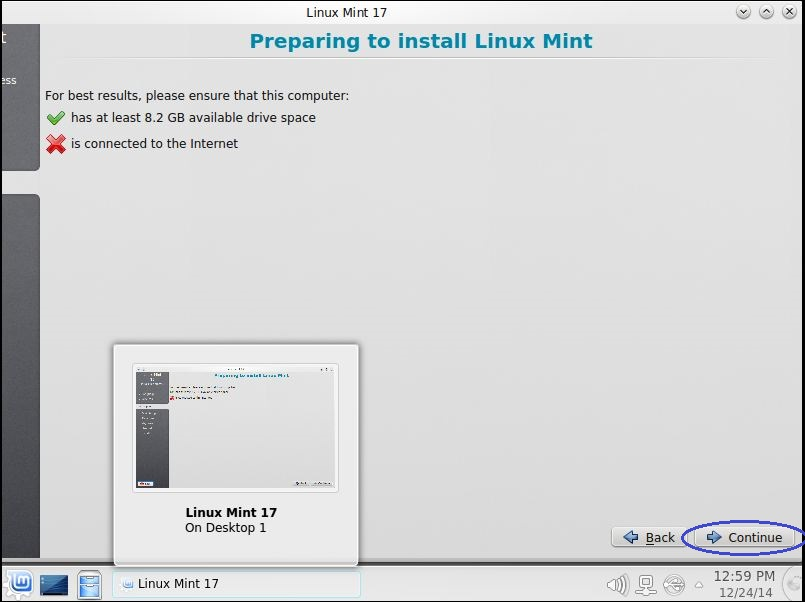
\includegraphics[width=14cm,height=9cm]{Capture3.JPG}
\end{center}
\newpage
5. Lalu pilih instalasi secara manual
\begin{center}
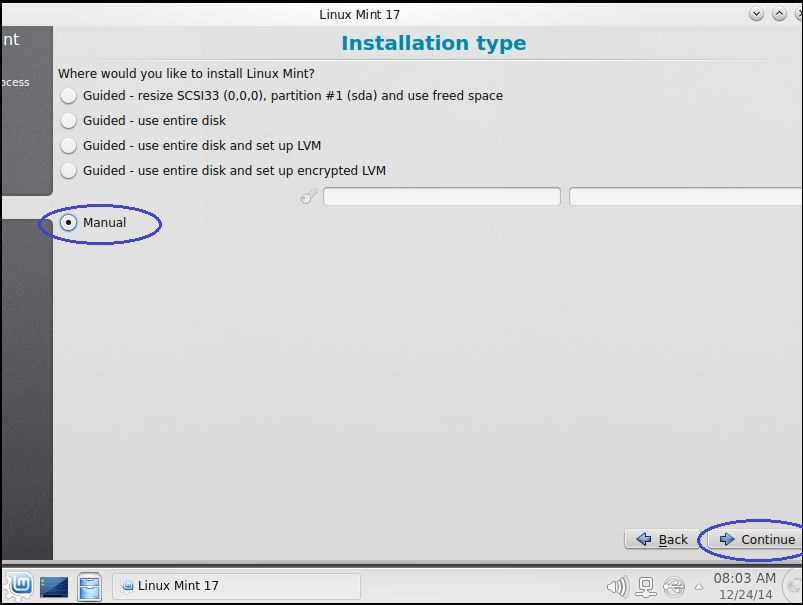
\includegraphics[width=14cm,height=9cm]{Capture5.JPG}
\end{center}
6. Lalu mempartisi free space (21474 MB) menjadi 3 bagian ext4 dengan mount point (/), swap,\\
\itab{\hspace{12pt}dan ext4 dengan mount point (home). ext4 adalah format disk pada linux, swap sebagai RAM}\\
\itab{\hspace{12pt}tambahan. Besar space untung ext4/ biasanya 3GB.}\\
\begin{center}
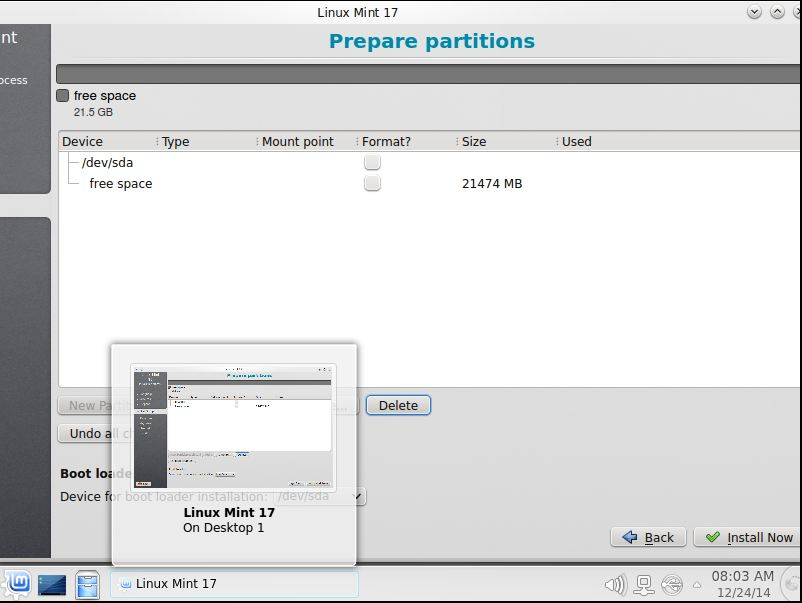
\includegraphics[width=14cm,height=9cm]{Capture6.JPG}\\
\end{center}
 \vspace{1cm}
\begin{center}
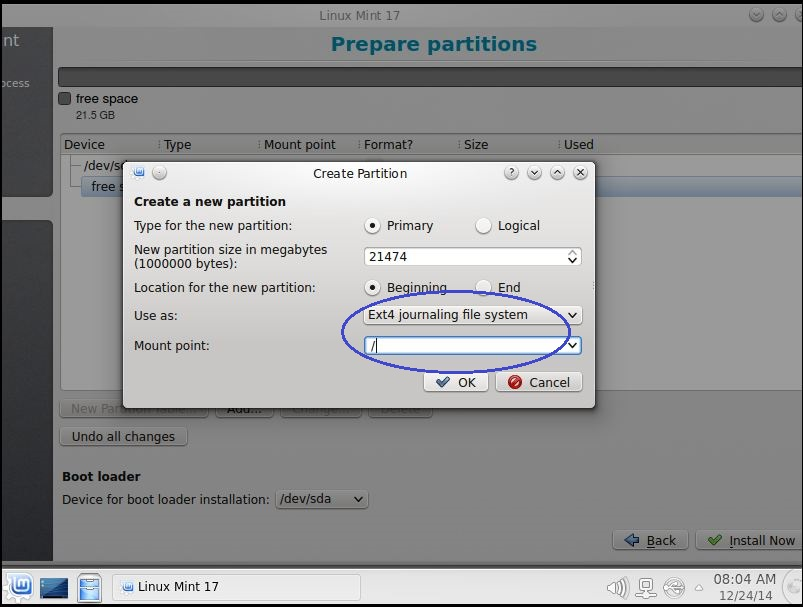
\includegraphics[width=14cm,height=9cm]{Capture7.JPG}\\
\end{center}
\begin{center}
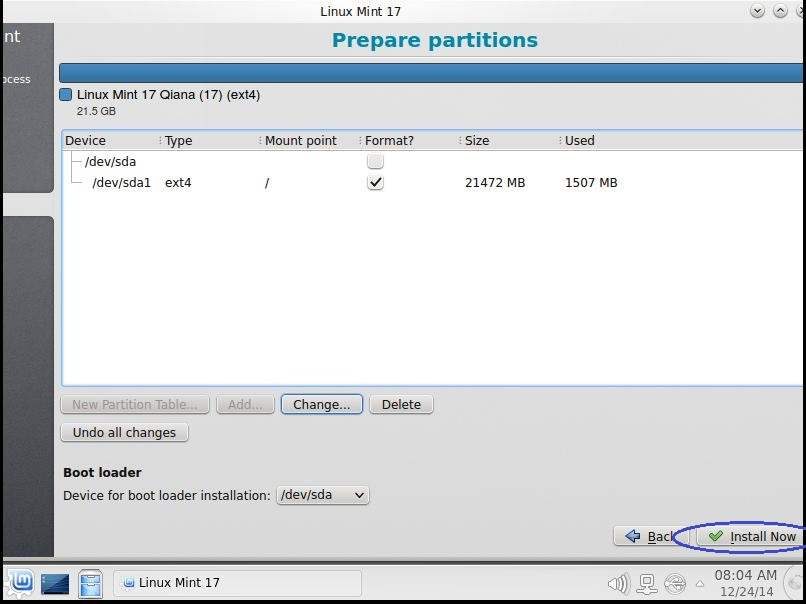
\includegraphics[width=14cm,height=9cm]{Capture8.JPG}\\
\end{center}
\newpage
7. Setelah itu klik pada peta untuk memilih time zone dimana anda berada.
\begin{center}
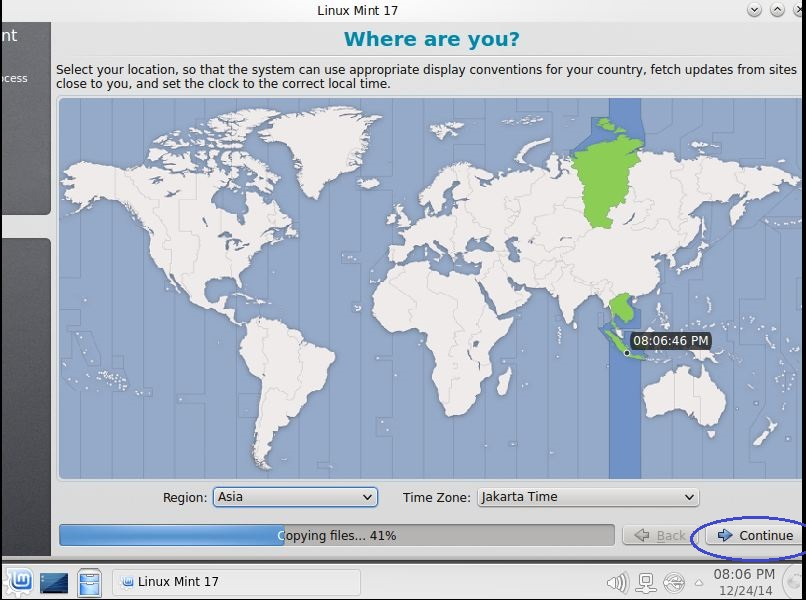
\includegraphics[width=14cm,height=9cm]{Capture9.JPG}\\
\end{center}
8. Setelah itu masukan keyboard layout English (US)
\begin{center}
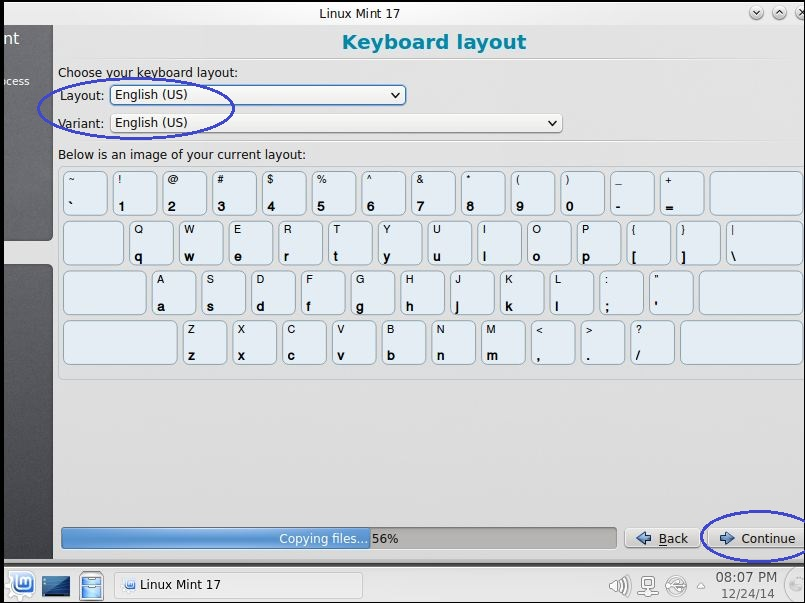
\includegraphics[width=14cm,height=9cm]{Capture10.JPG}\\
\end{center}
\newpage
9. Masukan nama dan password yang diinginkan seperti gambar dibawah ini
\begin{center}
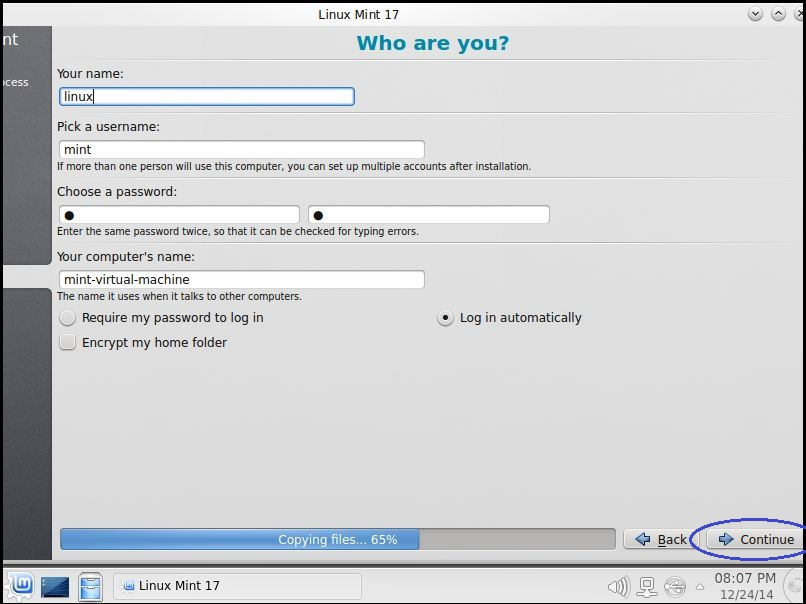
\includegraphics[width=14cm,height=9cm]{Capture11.JPG}\\
\end{center}
10. Selesai Menginstall Linux Mint 17 'Qiana`
\begin{center}
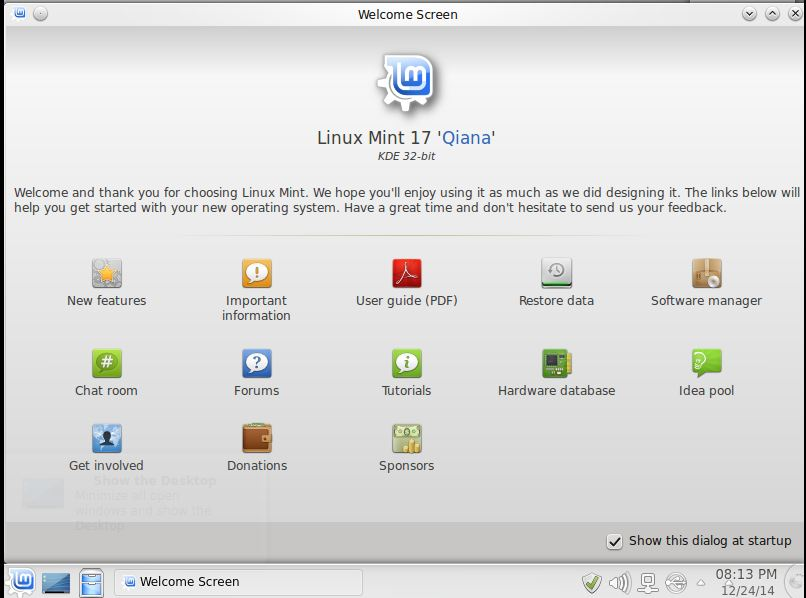
\includegraphics[width=14cm,height=9cm]{Capture12.JPG}\\
\end{center}
\end{document}


